\chapter{Logistik}
\label{Logistik}

\section{Einsatzgebiet \& Problemstellung}

Logistik gehört wie die Datenanalyse im Bereich von BigData zu den Problemgebieten, welche sich nicht so einfach lösen lassen. 
Grundsätzlich sind sie exakt mit genügend Zeit lösbar, aber nicht in der benötigten oder vorhandenen Zeit. 
Dieses Problem wirkt sich im 21. Jahrhundert stark aus, da immer mehr Güter transponiert werden und diese über die gesamte Welt. 
Am Beispiel des Paketdienstes UPS lässt sich dies erkennen. 
Im Jahr 2006 war das tägliche Zustellvolumen von Paketen und Dokumenten bei $14.1$ Millionen, im Jahr 2014 bereits bei $18.0$ Millionen\footnote{UPS - Weltweit, \url{https://www.ups.com/content/at/de/about/facts/worldwide.html}}. 
Dies entspricht einer Steigerung von $\sim27\,\%$, bei einer gleichzeitigen Erweiterung der Fahrzeugflotte um $\sim13\,\%$. 
Dies betrifft nicht nur Logistikunternehmen wie UPS, sondern auch zum Beispiel Brauereien, welche die Auslieferung ihrer Produkte nicht komplett ausgelagert haben. 

\noindent
Logistik beinhaltet mehr als nur Auslieferungen: 
\begin{itemize}
	\item Planung: Ein Disponent erstellt Listen an Aufträgen, die erledigt werden müssen;
	\item Organisation: Die Auftragslisten müssen einem Fahrzeug zugeteilt werden, wobei überprüft werden muss, ob die maximale Kapazität des Fahrzeugs nicht überschritten wird; 
	\item Steuerung: Die geplante Route kann vom Disponenten manuell oder durch ein Informationssystem automatisiert optimiert werden;
	\item Abwicklung: Erfolgt durch den Fahrer mit dem zugeteilten Fahrzeug; 
	\item Kontrolle: Durch Analyse der Touren und Fahrten kann ein Informationsrückfluss erfolgen, um den gesamten Prozess zu verbessern;
\end{itemize}

\noindent
Ein weiteres Problem betrifft die Anzahl der Stopps.
\begin{table}[htb]%[ht!]
\centering
\begin{tabular}{R{3cm}|R{3cm}|R{4cm}}
%\hline 
Anzahl der Haltepunkte & Anzahl der möglichen Routen & Berechnungszeit in Sekunden bei 30 Routen/Sekunde \\ 
\hline 
1 & 1 & 0.030 \\ 
%\hline 
2 & 2 & 0.067 \\ 
%\hline 
3 & 6 & 0.200 \\ 
%\hline 
4 & 24 & 0.800 \\ 
%\hline 
5 & 120 & 4.000 \\ 
%\hline 
6 & 720 & 24.000 \\ 
%\hline 
7 & 5.040 & 168.000 \\ 
%\hline 
8 & 40.320 & 1344.000 \\ 
%\hline 
9 & 362.880 & 12096.000 \\ 
%\hline 
10 & 3.628.800 & 120960.000 \\ 
%\hline 
11 & 39.916.800 & 1330560.000 \\ 
%\hline 
12 & 479.001.600 & 15966720.000 \\ 
%\hline 
13 & 6.227.020.800 & 207567360.000 \\ 
%\hline 
\end{tabular} 
\caption{Aufschlüsselung der Anzahl an möglichen Routen, gegeben durch die Berechnung der Fakultät der Anzahl an Knoten}
\label{tab:nfakult}
\end{table}
Wie in Tabelle \ref{tab:nfakult} ersichtlich, steigt die Anzahl der möglichen Routen mit der Anzahl der Stopps. 
Eine Route besteht hierbei aus einem Startdepot am Anfang und einem Enddepot am Ende. 
Zwischen diesen Punkten befinden sich mindestens ein Haltepunkt bis $n$ viele. 
Diese Anzahl lässt sich durch die Zahl der Stopps und dessen Fakultät berechnen. 
Daraus lässt sich ableiten, dass bis zu einem Grad alle Möglichkeiten testbar sind, abhängig von der Rechenleistung. 
Angenommen ein Rechner berechnet 30 Möglichkeiten pro Sekunde, so würde man bei 8 Stopps eine Zeit von $1344$ Sekunden bzw. $22,4$ Minuten benötigen. 

\subsection{Graph}

Graphen im Sinne der Logistik sind anders definiert als im Bereich der neuronalen Netzwerke. 
In der Graphentheorie ist ein Graph ein System an Knoten und Kanten. 
Dabei kann dieser als Paar $G := (V, E)$ interpretiert werden, welches aus zwei Mengen besteht. 
Eine Menge mit den Knoten $V$ und die zweite mit den Kanten $E$ zwischen den Knoten. 
Im Sinne der Graphentheorie kann entlang der Kanten durch den Graph navigiert werden. 

\noindent
Eine Spezialisierung bilden gerichtete Graphen, bei welchen die Kanten zusätzlich eine Richtung beinhalten. 
Des Weiteren existieren noch gewichtete Graphen mit Gewichtungen an den Kanten. 
Sie beschreiben, wie groß die Kosten sind, wenn die Kante zum Navigieren verwendet wird. 
Ein Beispiel dazu befindet sich in der Abbildung \ref{fig:graph}, mit 4 Knoten und einem voll vernetzten System zwischen diesen. 
Die Spezialisierungen der einzelnen Graphen-Typen können kombiniert werden, sowie um weitere Bedürfnisse abgeändert werden \cite{wurzer2010fallbeispiele}.
\begin{figure}
	\centering
	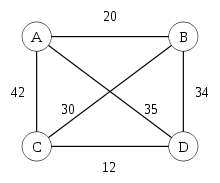
\includegraphics[scale=0.8]{images/220px-Weighted_K4.png}
	\caption{Beispiel für einen Graphen mit gewichteten Kanten und 4 Knoten als Kunden; Die Kosten sind dabei als ganze Zahlen an den Kanten angegeben; Bild: \url{www.wikipedia.org}}
	\label{fig:graph}
\end{figure}

\noindent
Um durch einen Graphen zu navigieren existieren Algorithmen, welche zum Beispiel die kürzeste Route von einem Punkt zu allen anderen im Graphen finden. 
Hierzu zählt zum Beispiel der Dijkstra-Algorithmus, der als Standardalgorithmus im Gebiet der kürzesten Routenfindung eingesetzt wird. 

\subsection{Traveling Salesman Problem (TSP)}

Das TSP oder auch unter dem Begriff \textit{Vehicel Routing Problem (VRP)} bekannt, stellt ein Grundproblem der Logistik dar. 
Bei dieser Problemstellung sollen geografische Positionen einmal angefahren werden und dies mit dem geringsten Aufwand. 
Dies lässt sich in der Abbildung \ref{fig:tsp} erkennen.
Dabei werden die größten Städte Deutschlands angefahren, der Start- und Zielpunkt sind dabei identisch. 
Dieses Problem kann mit einer Laufzeitkomplexität von $O((n-1)!/2)$ exakt gelöst werden, wobei mit zunehmender Größe des Faktors \textit{n}, die Berechnungszeit wesentlich größer wird. 
Aus diesem Grund wurden heuristische Algorithmen entwickelt, welche eine mögliche Lösung finden, aber sehr wahrscheinlich nicht die effizienteste Route. 
Heuristische Lösungen werden eingesetzt, da sie zeit- und ressourcensparender sind und dabei verwendbare Lösungen liefern \cite{wurzer2010fallbeispiele, laporte1992vehicle}. 
\begin{figure}
	\centering
	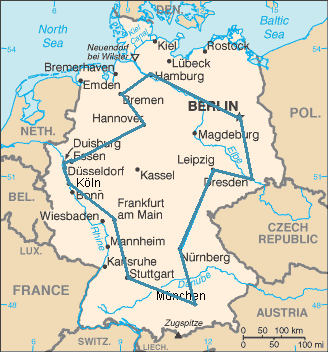
\includegraphics[scale=0.8]{images/TSP_Deutschland_3.png}
	\caption{Beispiel für eine Route durch Deutschland; Bild: \url{www.wikipedia.org}}
	\label{fig:tsp}
\end{figure}

\noindent
Weiters werden einige spezialisierte Formen des VRP kurz erklärt und beschrieben. 

\paragraph{Capacity Vehicle Routing Problem (CVRP):}

In dieser Erweiterung von VRP spielt besonders die Kapazität der Fahrzeuge eine Rolle, denn diese sollte so effizient wie möglich ausgenützt werden. 
Hierbei starten alle Fahrzeuge vom selben Depot, alle Kunden sind vorab bekannt. 
In diesem Fall besitzen alle Fahrzeuge dieselbe Kapazität, welche in der Route nicht überschritten werden darf \cite{laporte1992vehicle}. 

\noindent
Lösungsalgorithmen für CVRP:
\begin{itemize}
	\item Savings-Algorithmus: wird in Sektion \ref{savingKurz} erklärt 
	\item Der Sweep-Algorithmus verwendet ein \textit{Cluster-first} Vorgehen. 
	Hierbei werden Stopps einem Fahrzeug solange hinzugefügt, bis dessen Kapazität oder die maximale Routenlänge erreicht wird. 
	Die Zuteilung zu einem Fahrzeug wird durch Polarkoordinaten festgestellt und dessen Winkel zum aktuell ausgewählten Punkt. 
	Im Anschluss wird eine TSP Optimierung auf den erstellten Cluster an Haltepunkten ausgeführt und so eine optimierte Route generiert. 
	\item Ein \textit{Route-first} Vorgehen, wie von Beasley 1983 beschrieben, beginnt mit einer optimierten Route ohne Berücksichtigung der Nebenbedingungen. 
	Im Anschluss wird diese Route auf Fahrzeuge aufgeteilt, sodass die Nebenbedingungen eingehalten werden. 
\end{itemize} 

\paragraph{Periodic Vehicle Routing Problem (PVRP):}

PVRP stellt wie CVRP eine Erweiterung des Basisproblems dar. 
In diesem Fall sollen Kunden nicht einmal, sondern mehrmals angefahren werden. 
Dieses Problem tritt zum Beispiel bei einem Hausbau mit mehreren Betonlieferungen auf, über eine längere Zeit abhängig von der Nachfrage \cite{laporte1992vehicle}. 

\paragraph{Vehicle Routing Problem with Backhauls (VRPB):}

Das VRPB erweitert das CVRP um die Möglichkeit, Kunden nicht nur zu beliefern, sondern auch etwas entgegenzunehmen. 
Dabei entstehen zwei Teilmengen.
Kunden die beliefert werden und Kunden von welchen abgeholt werden soll. 
Im Grunde erweitert sich das Basismodell um eine Vorrangregel, bei welcher zu beliefernde Kunden bevorzugt werden. 
Ansonsten könnte der Fall eintreten, dass ein Fahrzeug keine Zusatzladung mehr aufnehmen kann \cite{wurzer2010fallbeispiele}.

\paragraph{Vehicle Routing Problem with Time Windows (VRPTW):}

Das VRPTW erweitert ebenfalls das CVRP, sodass Kunden nicht zu jeder Zeit angefahren werden können.
Dieses Problem ist aus der Praxis heraus gewachsen, denn manche Kunden und Lager sind nur zu bestimmten Zeiten anzutreffen. 
Zusätzlich könnten Straßensperren berücksichtigt werden, wie zum Beispiel eine Innenstadt mit Zustellungserlaubnis am Vormittag. 
Das Basismodell muss hierbei um Zeitintervalle erweitert werden, weiters müssen die Abfahrtszeiten vom Depot, Fahrzeiten für alle Teilstrecken und Servicezeit bei jedem Kunden vorhanden sein. 
Im Gesamten muss festgelegt werden wie optimiert werden soll, denn es besteht die Möglichkeit, dass Fahrzeuge warten müssen, bis der Kunde anzutreffen ist. 
Im Falle einer Wartezeit könnte zuerst ein anderer Kunde angefahren werden. 
Dies bedeutet, dass wahrscheinlich eine längere Strecke zurückgelegt werden muss \cite{wurzer2010fallbeispiele}. 

\noindent
Lösungsalgorithmen für VRPTW:
\begin{itemize}
	\item Savings-Algorithmus
	\item Route-first, Cluster-second (Solomen 1986)
	\item Sequentielle Einfügeheuristik (Solomon 1987)
	\item Zeitorientierte Nearest-Neighbor Heuristik 
	\item Tabu-Search
	\item Evolutionäre Algorithmen
\end{itemize} 

\paragraph{Pick-up-and-delivery Problem (PDP):}

Das PDP stellt eine zusätzliche Spezialisierung des VRP dar. 
In diesem Fall müssen Abholungen und Lieferungen in einer Route erledigt werden. 
Dabei ist die Kapazität der Fahrzeuge sehr zu berücksichtigen, da diese erst wieder zusätzliche Ladungen aufnehmen können, wenn genügend Kapazität dafür vorhanden ist. 
Außerdem muss berücksichtigt werden, dass eine Ladungsaufnahme in dieser Route später auch zugestellt wird. 
Diese Ladungen dürfen nicht als Auslieferung für eine weitere Route übernommen werden. \\

\noindent
Diese Beschreibungen stellen nur eine Teilmenge der Problemdomänen dar, weshalb für genauere Informationen Fachlektüre hinzugezogen werden sollte. 
Des Weiteren existieren Meta-Heuristische Algorithmen, welche eine geringe Laufzeit besitzen, dafür kein exaktes Ergebnis liefern, sondern nur eine Annäherung. 

\section{Lösungsverfahren}

\subsection{Exakte Verfahren}

Exakte Verfahren liefern die beste Lösung, aber nicht ohne Nachteile.  
Einer dieser Nachteile ist, dass die benötigte Zeit mit jedem weiteren Knoten im System stark ansteigt, da die zu überprüfenden Möglichkeiten  steigen. 

\paragraph{Branch-and-Cut:}	

\textit{Branch-and-Cut} vereint zwei Verfahren, welche ebenfalls im Gebiet der Logistik eingesetzt werden: Das Schnittebenenverfahren und das \textit{Branch-and-Bound} Verfahren. 
Ziel dieser ganzzahligen linearen Optimierung stellt eine lineare Zielfunktion dar, welche gesucht wird. 
Diese Funktion wird mit Hilfe von linearen Ungleichungen gesucht, welche eine Menge an Punkten umschließen. 
Durch das Schnittebenenverfahren werden weitere Ungleichungen in das System eingefügt, welche von allen zulässigen Punkten erfüllt werden. 
Durch ein weiteres Lösen des Systems muss eine neue Lösung entstehen, welche näher am gesuchten Optimum liegt.
Das \textit{Branch-and-Bound} wird im Anschluss ausgeführt, wenn keine Schnittebenen mehr gefunden werden. 
Die genauere Beschreibung dieses Algorithmus befindet sich in der Sektion \ref{Heuristik}, da dieses Verfahren in der Fachliteratur den Übergruppen \textit{exakte Verfahren} und \textit{heuristische Verfahren} zugeordnet wird. 

\subsection{Heuristik}
\label{Heuristik}

Heuristik bedeutet, mit wenig Wissen sowie mit begrenzter Zeit eine wahrscheinliche Lösung zu liefern. 
Heuristiken werden oft im Gebiet der Optimierungen eingesetzt. 
Zum exakten Lösen eines Logistik-Problems wird sehr viel Zeit und Speicher benötigt. 
Deshalb werden hier häufig Heuristiken eingesetzt. 
Ein Vorteil der Heuristik ist es, dass in kurzer Zeit gute Lösungen für schwierige Probleme gefunden können. 
Die Nachteile dieser Methoden sind aber nicht zu vernachlässigen, sie geben nämlich:
\begin{itemize}
	\item keine Garantie für die optimale Lösung;
	\item keine Garantie für eine Lösung und für die Güte einer Lösung;
\end{itemize}

\paragraph{Branch-and-Bound:}

Im Grunde wird bei diesem Algorithmus ein Baum im Sinne der Informationstechnologie aufgebaut, in welchem anhand der Möglichkeiten gesucht und verglichen wird. 
Dabei werden Schwellenwerte für die Kosten festgelegt, welche bei einer Route nicht über- und unterschritten werden dürfen.
\begin{itemize}
	\item \textit{Branchen} (Verzweigung) ist der erste Schritt in diesem Algorithmus. 
	Hierbei wird das Problem in mehrere Teilprobleme aufgeteilt und in einer Baumstruktur abgelegt. 
	\item \textit{Bounden} (Beschränkung) repräsentiert den zweiten Schritt, in welchem die Lösungsmenge beschränkt wird. 
	Dabei wird überprüft, welche Zweige suboptimal sind und als mögliche Lösungen verworfen werden. 
\end{itemize}
Eine Lösung wird verworfen, wenn das Gewicht eines \textit{1-tree} größer ist als das Gewicht einer zuvor gefundenen möglichen Lösung. 
Ein \textit{1-tree} beschreibt dabei einen Weg von der Hauptwurzel bis zu einem Endblatt. 
Diese Art der Routenfindung liefert rasch brauchbare Ergebnisse \cite{wiener2003branch}. 

\paragraph{Nearest-Neighbor (NN):}

Die NN-Heuristik stellt ein mögliches Eröffnungsverfahren dar. 
Diese liefert zwar eine Approximation der Lösungen, aber meist nicht sehr gute Resultate. 
Der Algorithmus kann dazu verwendet werden, um eine Beispiellösung zu generieren. 
Diese Lösung kann als Ausgangszustand für Verbesserungsheuristiken eingesetzt werden, welche selbst keine Grundlösung finden würden. 
Der Grundalgorithmus wählt zufällig einen Knoten aus dem System und sucht sich anhand diverser Kriterien einen weiteren Knoten, welcher als \textit{Nearest-Neigbor} bezeichnet wird. 
Von diesem ausgehend wird ein weiterer Knoten zur Route hinzugefügt, bis diese vollständig ist. 
Ein Nachteil dieses Algorithmus lässt sich am Ende erkennen, wenn die Route vollständig ist.
Start und Endpunkt liegen oft sehr weit auseinander. 
Dieses Verhalten ist meist nicht gewünscht, da eine Rundreise erwartet wird und nicht eine Route im Sinne einer Linie und einem langen Rückweg \cite{jp2010opttrans}. 

\noindent
Von diesem Algorithmus aus existieren noch einige weitere Spezialisierungen, wie zum Beispiel der \textit{Variable Neighbourhood Search} Algorithmus.
Dieser nützt den Vergleich von lokalen Optima zu globalen Optima, um effizientere Routen zu finden. 

\paragraph{Savings-Algorithmus (SA):} 
\label{savingKurz}

Der SA von Clarke und Wright gehört nicht zur Kategorie der Eröffnungsverfahren, sondern zu den Optimierungsalgorithmen. 
Bei diesem wird hauptsächlich mit einem Saving gearbeitet. 
Dieses Saving repräsentiert, wie viel gespart werden kann, wenn der Kunde \textit{B} nach dem Kunden \textit{A} angefahren wird und somit zwischen diesen Kunden nicht zum Depot zurückgekehrt werden muss. 
Dabei spielt die Berechnung des Savings aus den Kosten eine wichtige Rolle, auf welche später noch genauer eingegangen wird. 

\noindent
Der Algorithmus beruht darauf, in jedem Schritt eine Route zu vergrößern und dabei einige andere zu entfernen. 
Der grundsätzliche Ablauf sieht wie folgt aus:
\begin{enumerate}
	\item Zu Beginn müssen Werte zur Berechnung der Ersparnisse initialisiert werden, wie eine Zeit- oder Distanzmatrix. 
	In diesem Schritt wird aus jedem Knoten/Kunde eine triviale Route erstellt, bestehend aus \textit{Depot - Knoten - Depot}.
	\item Im nächsten Schritt wird jede Route mit jeder anderen Route gepaart und der Savings-Wert berechnet. 
	In diesem Schritt muss auch überprüft werden, ob die Kombinationen die Nebenbedingungen einhalten. 
	Sollte dies nicht der Fall sein, muss diese Möglichkeit verworfen werden. 
	\item Die Kombination von zwei Routen mit dem höchsten Saving, wird im Anschluss zu einer neuen Route vereint. 
	\item Nach der Kombination müssen alle Möglichkeiten entfernt werden, welche die zweite Teilroute beinhalten. 
	Zusätzlich müssen alle Teilrouten mit dem ersten Teil durch die neue Route ersetzt werden. 
	\item Infolgedessen wird bei Punkt 2 fortgesetzt, wenn sich noch Kombinationen an Routen in der Savingsliste befinden. 
	Sollte dies nicht der Fall sein, so wurde eine optimierte Route gefunden oder mehrere Teilrouten, welche nicht mehr kombiniert werden können. 
\end{enumerate}

\paragraph{Sweep-Algorithmus:}

Der Sweep-Algorithmus verwendet wie zuvor schon erwähnt ein \textit{Cluster-first} Vorgehen. 
Dieser verwendet ein geometrisches Verfahren zum Erstellen des Clusters, weshalb dieser nur in planaren Instanzen angewendet werden kann.
Jeder Kunde im System wird in einem Polarkoordinatensystem repräsentiert. 
Jeder besitzt einen Winkel und einen direkten Abstand zum zentralen Depot. 
\begin{itemize}
	\item Zu Beginn wird ein beliebiger Knoten/Kunde als erster Haltepunkt in der Route ausgewählt.
	\item Im Anschluss wird zu diesem Ausgangspunkt ein weiterer Kunde hinzugefügt und zwar dieser mit dem geringsten Winkelabstand zum letzten Punkt in der Route. 
	\item Dieser Prozess wird solange durchgeführt, bis eine Route eine maximale Anzahl an Punkten erreicht hat oder ein Fahrzeug keine Kapazität mehr zur Verfügung hat. 
	\item Damit wurde ein Cluster an Stopps für ein Fahrzeug erstellt, welcher im einem zweiten Schritt zu einer optimierten Route entwickelt werden muss. 
\end{itemize}
Somit gehört auch dieser Algorithmus zur Kategorie der Eröffnungsverfahren \cite{jp2010opttrans}. 

\subsection{Meta-Heuristiken}

Meta-Heuristik wird in der Informatik als Bezeichnung verwendet, wenn eine Lösung näherungsweise erzeugt wird. 
Diese sind nicht stark problemspezifisch orientiert, im Gegensatz zu Heuristiken. 
Diese Art von Algorithmen wird im Bereich der Logistik deshalb eingesetzt, weil sie lokalen Optima in schwereren und größeren Problemen entwischen können und eher zu einem globalen Optima tendieren oder konvergieren. 

\paragraph{Tabu-Search (TS):}

Der \textit{Tabu-Search} baut auf keiner bisher beschriebenen Methode auf. 
Im Unterschied zu anderen Algorithmen sind beim TS auch ungültige Lösungen zugelassen, welche die Nebenbedingungen verletzen. 
Es muss dafür eine Kostenfunktion existieren, mit welcher die Kosten einer Lösung festgestellt werden können. 
Für jede gefundene Lösung wird evaluiert, ob dies eine verwendbare Lösung ist oder nicht. 
Hierbei fließen die einzelnen Nebenbedingungen, mit einem hinzumultiplizierten Faktor, eine Rolle. 
So kann festgestellt werden, ob es sich um eine bessere Lösung handelt oder nicht. 
Eine Kernfunktionalität stellt die Tabu-Liste dar. 
In dieser werden Unmöglichkeiten gespeichert, welche nicht durchgeführt werden dürfen, solange sie sich in der Liste befinden. 
Zum Beispiel darf von einem Ort aus nicht nach Osten zum nächsten gefahren werden, da dieser Zug in der Iteration vorher durchgeführt worden ist. 

\noindent
Der Hauptalgorithmus besteht aus einer Hauptschleife, welche an ein Abbruchkriterium geknüpft ist. 
Zu Beginn wird dabei eine mögliche Lösung initialisiert und als aktuell beste Lösung angenommen. 
Im Anschluss werden weitere mögliche Lösungen erzeugt und die Beste daraus ausgewählt. 
Diese alternative Lösung wird mit der aktuell besten Lösung verglichen und als neue Beste definiert, wenn dies der Fall ist. 
Daraufhin wird die Tabu-Liste aktualisiert. 
Dieser Ablauf wird solange durchgeführt, bis das Abbruchkriterium eintritt.

\noindent 
Bei diesem Algorithmus wird nicht garantiert, dass eine gültige Lösung gefunden wird. 
So kann aber eine Lösung entstehen, welche weit geringere Kosten mit sich bringt als eine Lösung ohne Verletzung der Nebenbedingungen. 
Im Falle einer Applikation muss durch die Evaluierungsfunktion definiert sein, in wie weit eine Nichteinhaltung toleriert wird oder nicht \cite{jp2010opttrans}. 

\paragraph{Simulated Annealing (SA):} 

SA ist für sich im Detail kein Algorithmus, sondern bezeichnet eine Klasse von Algorithmen, welche versuchen global zu optimieren. 
Die Idee und die Bezeichnung stammen hierbei aus der Härtung von Stahl. 
In der Stahlproduktion wird dieser \textit{erwärmt} und wieder \textit{abgekühlt}, was als \textit{härten} bezeichnet wird. 
Dieser Prozess des Abkühlens führt dazu, dass sich die Teilchen wie in einer Gitterstruktur anordnen. 
Zu Beginn kann von einer stochastischen Suche gesprochen werden und zum Ende hin von einer deterministischen Suche. 
Zum Ende des Prozesses werden die Schritte immer kleiner, wie bei der Härtung kühlen dabei die letzten Temperaturen sehr langsam ab. 
Im Gesamten wird eine global optimale Konfiguration gefunden, in dem dieser Prozess simuliert wird. 
Am Anfang wird deshalb von einer stochastischen Suche gesprochen, da das System Möglichkeiten annimmt, welche zu einer Verschlechterung des Ergebnisses führen. 
Wird die sogenannte Temperatur geringer, minimiert sich die Akzeptanz für Möglichkeiten, was wiederum deterministisch ist. 
Der stochastische Anteil ermöglicht dem lokalen Minima zu entkommen und dem globalen Minima sich anzunähern. 
Der Grundalgorithmus ähnelt dabei sehr dem \textit{Tabu-Search} mit der Hauptschleife. 
Beim SA wird solange optimiert, bis das System einen erstarrten Zustand erreicht \cite{kirkpatrick1983optimization}. 

\paragraph{Ant Colony Optimierung (ACO):}

ACO repräsentiert eine Simulation von sozialen Interaktionen in der Natur.
So wurde für diesen Algorithmus das Verhalten und die Interaktionen von Ameisen, Bienen und weiteren Insekten analysiert. 
Jedes Individuum dieser Insekten erledigt eine eigene Aufgabe, unabhängig von anderen in der Kolonie. 
Ein funktionierendes System kommt dadurch zustande, dass die Arbeiten jedes einzelnen Individuums auf den Arbeiten eines anderen aufbauen oder mit anderen verbunden sind.
Durch die Kooperation in der Kolonie, entsteht die Möglichkeit, komplexe Probleme zu lösen und Überlebensstrategien auszuführen \cite{mucherino2015ant, abraham2006swarm}. 

\noindent
Damit dieser Algorithmus eingesetzt werden kann, müssen einige Grundvoraussetzungen erfüllt sein:
\begin{itemize}
	\item Eine Strategie zum Überprüfen einer gültigen Lösung, damit nur solche akzeptiert werden;
	\item Eine heuristische Funktion $\eta$ zum Messen der Qualitäten der Teile, welche sich noch nicht in der Teillösung befinden;
	\item Eine Funktion zum Aktualisieren der Pheromone $\tau$, welche die Wertigkeit der Kanten repräsentiert; 
	\item Eine Funktion $\phi$, welche auf der heuristischen Funktion $\eta$ und den Pheromonen aus $\tau$ basiert und iterativ mögliche Lösungen konstruiert;  
\end{itemize}

\noindent
Der grobe Ablauf des Grundalgorithmus: 
\begin{itemize}
	\item Zu Beginn wird die Ameise an einem Startpunkt ausgesetzt;
	\item Diese besitzt nun die Möglichkeit sich mit einer bestimmte Anzahl von Zügen durch das Netzwerk zu bewegen unter Berücksichtigung der Funktion $\phi$; dabei wird eine Tabu-Liste für diese Ameise erstellt; 
	\item Im Anschluss wird die Tour der Ameise bewertet und
	die Pheromone der Kanten berechnet; eine weitere Ameise wird ausgesetzt bis die maximal Anzahl der Ameisen erreicht ist;
	\item Nachdem alle Ameisen einmal im Netzwerk waren, werden alle Pheromone an den Kanten aktualisiert; 
	\item Diese entstandene Lösung wird nun mit der letzten verglichen und ein weiterer Durchlauf wird unter Berücksichtigung eines Abbruchkriteriums mit den neuen Pheromonen eingeleitet; 
\end{itemize}

\paragraph{Evolutionäre Algorithmen (EA):}

EA sind wie SA kein Algorithmus, sondern ein Überbegriff für eine Klasse von Algorithmen und Methoden. 
Das Prinzip dieser Algorithmen beruht auf dem Vorgang einer biologischen Evolution. 
Die Natur einer biologischen Evolution ist es, sich zu verbessern und zu überleben, was äquivalent zu einem Optimierungsprozess ist. 
In der Natur sind die Vorgänge der Optimierung bei einem Menschen sehr langsam und für ein einzelnes Individuum nicht wahrnehmbar. 
Dabei muss sich jede Generation aufs Neue behaupten und beweisen, dass sie mit der aktuellen Umgebung besser zurechtkommt. 
Diese Selektion geschieht ganz nach \textit{Charles Darwins} Worten \textit{survival of the fittest}, sodass der Angepassteste/Fitteste sich am stärksten verbreitet beziehungsweise vermehrt. 
Die Veränderungen entstehen dabei durch einfache Fortpflanzung im Sinne einer Rekombination und durch Mutationen. 
So wird bei der Mutation nur ein Individuum benötigt, welches verändert wird und bei der Rekombination zwei. 

\noindent
Ein EA besitzt genau solche Eigenschaften und versucht hier die Natur nachzuahmen. 
Im Sinne eines Algorithmus werden die Rekombination und Mutation schneller durchgeführt, sodass immer Mengen an potentiellen Lösungen zur Verfügung stehen. 
Alle Lösungen werden evaluiert und ihre Fitness bestimmt. 
Unbrauchbare Lösungen werden aussortiert, wenn sie nicht fit genug sind, bis eine geeignete Lösung gefunden wurde oder ein Abbruchkriterium wirksam wird \cite{isl2008ea, beyer2001evolution}. 

\noindent
Der grundsätzliche Ablauf sieht wie folgt aus:
\begin{enumerate}
	\item Zu Beginn muss eine Beispiellösung initialisiert und bewertet werden, um einen Ausgangszustand zu erlangen; 
	\item Im Anschluss wird eine Selektion durchgeführt; 
	\item Die Selektierten werden rekombiniert und so Nachkommen erzeugt; 
	\item Auf die gesamte Menge an Lösungen wird eine Mutation angewendet; 
	\item Zum Abschluss werden alle Lösungen bewertet und ihre Fitness wird festgestellt;
	\item Sollte kein Abbruchkriterium erfüllt sein, so wird ab Punkt 2 wieder fortgesetzt; 
\end{enumerate}

\noindent
In diesem Kapitel wurden grundlegende Eigenschaften in der Logistik erklärt und Problemgebiete aufgezeigt. 
Es wurden einige Lösungsansätze beschrieben, um deren Grundalgorithmus zu verstehen. 
Im nächsten Kapitel wird auf Kostenfunktionen eingegangen und Probleme darin aufgezeigt. 